\documentclass[conference]{IEEEtran}
\IEEEoverridecommandlockouts
\usepackage{cite}
\usepackage{amsmath,amssymb,amsfonts}
\usepackage{algorithmic}
\usepackage{graphicx}
\usepackage{textcomp}
\usepackage{xcolor}
\usepackage{hyperref}
\usepackage{bookmark}
\usepackage{booktabs}
\usepackage{array}
\usepackage{listings}
\usepackage{makebox}

\begin{document}

\title{Effect of Screen Time on Quality of Sleep: Introductory Data Analysis Project Report\\

\large\color{blue} \href{https://github.com/abdulhanan1000/effect-of-screen-time-on-sleep-quality-IDA-project-main}{GitHub Repository With LaTeX and R Code (Click Here or View End Of Doc)}}

\author{
    \IEEEauthorblockN{1\textsuperscript{st} Abdul Hanan Javaid}
    \IEEEauthorblockA{\textit{MSc High Integrity Systems} \\ \textit{Frankfurt UAS} \\ \small Email: abdul.javaid@stud.fra-uas.de \\ Matriculation Number: 1541621 \\ Contributions: Code, Model, Background\\ and Literature Review, Results,\\ Limitations, Recommendations, \\ Conclusion, Acknowledgments,\\ Overall Project Group Work}
    \and
    \IEEEauthorblockN{2\textsuperscript{nd} Muhammad Saad Zafar}
    \IEEEauthorblockA{\textit{MSc High Integrity Systems} \\ \textit{Frankfurt UAS} \\ \small Email: muhammad.zafar@stud.fra-uas.de \\ Matriculation Number: 1541717 \\ Contributions: Data Collection, Abstract,\\ Research Design, Future Work,\\Discussion, Overall Project Group Work}
    \and
    \IEEEauthorblockN{3\textsuperscript{rd} Tehreem Iftikhar}
    \IEEEauthorblockA{\textit{MSc High Integrity Systems} \\ \textit{Frankfurt UAS} \\ \small Email: tehreem.iftikhar@stud.fra-uas.de \\ Matriculation Number: 1541382 \\ Contributions: Research Questions,\\ References, Discussion, \\ Overall Project Group Work }
}


\maketitle
\begin{abstract}
    This study examines how screen time before bed affects sleep quality. We collected data from 30 participants and used logistic regression to analyze the relationship between screen time and sleep quality. The results show that spending more than 2 hours on screens before bed is linked to poorer sleep quality. These findings suggest that reducing screen time before bed could improve sleep quality.
\end{abstract}

\section{Introduction}
\subsection{Context and Motivation}
The digital revolution has basically transformed human behavior patterns, particularly in the crucial hours before sleep. The use of smartphones, tablets, and computers has led to alarming levels of screen exposure, raising significant concerns about its impact on sleep quality and overall health.

\subsection{Research Objectives}
This study aims to:
\begin{itemize}
\item Quantify the relationship between before bedtime screen exposure and sleep quality
\item Identify potential threshold effects in screen time duration
\item Develop evidence-based recommendations for optimal screen time management
\item Contribute to the broader understanding of digital wellness
\end{itemize}

\subsection{Research Questions}
Primary research questions include:
\begin{itemize}
\item RQ1: What is the quantitative relationship between pre-bedtime screen time and sleep quality?
\item RQ2: Is there a critical threshold of screen time beyond which sleep quality significantly deteriorates?
\item RQ3: What are the implications for developing effective sleep hygiene interventions?
\end{itemize}

\section{Background and Literature Review}
\subsection{Theoretical Framework}
The relationship between screen exposure and sleep quality is grounded in several theoretical frameworks:

\subsubsection{Circadian Rhythm Theory}
Research has shown that exposure to blue light from digital devices can suppress melatonin production, disrupting the natural circadian rhythm. Studies by Chang et al. (2015) demonstrated earlier that blue light exposure can delay the production of melatonin by up to 3 hours \cite{chang2015}.

\subsubsection{Sleep Hygiene Model}
Traditional sleep hygiene models are being revised to incorporate the challenges posed by digital device usage, suggesting the need for updated guidelines that account for modern technology use patterns \cite{cajochen2011}.

\subsection{Previous Research}
Recent studies have identified several key mechanisms through which screen time affects sleep:

\subsubsection{Physiological Mechanisms}
\begin{itemize}
\item Blue light exposure affecting melatonin production \cite{chang2015}
\item Increased cognitive arousal and neural activation \cite{heath2014}
\item Altered sleep-wake cycle regulation \cite{cajochen2011}
\item Changes in core body temperature patterns
\end{itemize}

\subsubsection{Psychological Mechanisms}
\begin{itemize}
\item Content-induced emotional arousal
\item Fear of missing out (FOMO)
\item Digital anxiety and stress
\item Delayed sleep onset due to engagement
\end{itemize}

\section{Methodology}
\subsection{Research Design}
\subsubsection{Study Type}
This research employed a cross-sectional observational design with quantitative analysis. The design was chosen to:
\begin{itemize}
\item Capture current patterns of screen use and sleep quality
\item Enable statistical modeling of relationships
\item Facilitate comparison across demographic groups
\item Allow for robust statistical inference
\end{itemize}

\subsubsection{Sampling Strategy}
Participants were recruited using:
\begin{itemize}
\item Stratified random sampling within the population
\item Voluntary participation with informed consent
\item Inclusion/exclusion criteria based on screen time usage
\end{itemize}

\subsection{Data Collection}
\subsubsection{Participant Demographics}
Detailed demographic distribution:
\begin{table}[htbp]
\begin{center}
\begin{tabular}{|l|c|c|}
\hline
\textbf{Characteristic} & \textbf{Count} & \textbf{Percentage} \\
\hline
\multicolumn{3}{|l|}{\textbf{Gender}} \\
Male & 24 & 80\% \\
Female & 6 & 20\% \\
\hline
\multicolumn{3}{|l|}{\textbf{Age Groups}} \\
23-24 years & 10 & 33.3\% \\
25-26 years & 14 & 46.7\% \\
27-28 years & 6 & 20\% \\
\hline
\end{tabular}
\end{center}
\caption{Demographic Distribution of Study Participants}
\end{table}

\subsubsection{Data Collection Instruments}
The study utilized:
\begin{itemize}
\item Structured self-report questionnaires
\item Digital time-tracking logs
\item Sleep quality assessment forms
\item Demographic information sheets
\end{itemize}

\subsubsection{Variable Measurement}
\paragraph{Independent Variable}
Screen time was measured with the following parameters:
\begin{itemize}
\item Temporal resolution: 30-minute intervals
\item Measurement period: Last hour before sleep
\item Device types included: Smartphones, tablets, computers
\item Self-reported with standardized logging format
\end{itemize}

\paragraph{Dependent Variable}
Sleep quality was assessed using:
\begin{itemize}
\item Binary classification (Good/Bad)
\item Standardized sleep quality criteria
\item Multiple assessment points
\item Validated self-report measures
\end{itemize}

\subsection{Statistical Analysis}
\subsubsection{Statistical Methods}
Primary analysis methods included:
\begin{itemize}
\item Descriptive statistics
\item Logistic regression modeling
\item Odds ratio calculation
\item Confidence interval estimation
\item Model diagnostics
\item ROC curve analysis
\item Sensitivity and specificity calculation
\end{itemize}

\subsubsection{Model Specification}
The logistic regression model was specified as:

\begin{equation}
\log\left(\frac{p}{1-p}\right) = \beta_0 + \beta_1X + \epsilon
\end{equation}

Where:
\begin{itemize}
\item p = probability of good sleep quality
\item X = screen time before bed (hours)
\item $\beta_0$ = intercept
\item $\beta_1$ = coefficient
\item \(\epsilon\) = error term
\end{itemize}

\section{Results}
\subsection{Descriptive Analysis}
\subsubsection{Screen Time Distribution}
The screen time distribution among participants is summarized in Table \ref{tab:screen_time_distribution}.

\begin{table}[htbp]
\begin{center}
\begin{tabular}{|l|c|}
\hline
\textbf{Statistic} & \textbf{Value} \\
\hline
Mean & 2.08 hours \\
Median & 2.00 hours \\
Standard Deviation & 0.82 hours \\
Range & 0.5 - 4.0 hours \\
\hline
\end{tabular}
\end{center}
\caption{Screen Time Distribution Statistics}
\label{tab:screen_time_distribution}
\end{table}

\subsubsection{Sleep Quality Patterns}
\begin{itemize}
\item Overall distribution: 50\% good, 50\% bad
\end{itemize}

\subsubsection{Sleep Data}
The data collected from the participants is shown in Table \ref{tab:sleep_data}.

\begin{table}[htbp]
\begin{center}
\begin{tabular}{|l|c|c|c|}
\hline
\textbf{Gender} & \textbf{Age} & \textbf{Screen Time (hours)} & \textbf{Sleep Quality} \\
\hline
Male & 26 & 2.5 & Good \\
Male & 24 & 2.0 & Good \\
Male & 26 & 1.0 & Bad \\
Female & 24 & 3.0 & Good \\
Male & 26 & 3.0 & Good \\
Male & 26 & 1.0 & Good \\
Male & 25 & 2.0 & Good \\
Male & 27 & 3.0 & Bad \\
Male & 24 & 2.0 & Bad \\
Male & 24 & 2.0 & Bad \\
Female & 26 & 2.0 & Good \\
Male & 24 & 1.0 & Bad \\
Female & 25 & 2.5 & Bad \\
Female & 24 & 2.0 & Bad \\
Male & 25 & 3.0 & Bad \\
Male & 26 & 2.0 & Good \\
Male & 23 & 3.0 & Bad \\
Male & 27 & 2.0 & Bad \\
Male & 28 & 1.0 & Good \\
Male & 25 & 2.0 & Bad \\
Male & 27 & 1.0 & Good \\
Male & 26 & 0.5 & Good \\
Male & 25 & 1.0 & Good \\
Male & 24 & 2.0 & Good \\
Male & 24 & 4.0 & Bad \\
Male & 24 & 3.0 & Bad \\
Male & 26 & 2.0 & Good \\
Male & 25 & 3.0 & Good \\
Male & 27 & 2.0 & Good \\
Male & 24 & 2.0 & Bad \\
\hline
\end{tabular}
\end{center}
\caption{Sleep Data Collected from Participants}
\label{tab:sleep_data}
\end{table}

\subsection{Logistic Regression Results}
\subsubsection{Model Fit Statistics}
The logistic regression model fit statistics are as follows:
\begin{itemize}
\item Null deviance: 41.455 on 29 degrees of freedom
\item Residual deviance: 39.092 on 28 degrees of freedom
\item AIC: 43.092
\end{itemize}

\subsubsection{Parameter Estimates}
The parameter estimates for the logistic regression model are presented in Table \ref{tab:parameter_estimates}.

\begin{table}[htbp]
\begin{center}
\begin{tabular}{|l|c|c|c|c|}
\hline
\textbf{Variable} & \textbf{Coefficient} & \textbf{SE} & \textbf{z-value} & \textbf{p-value} \\
\hline
Intercept & 1.674 & 1.128 & 1.484 & 0.138 \\
Screen Time & -0.735 & 0.503 & -1.460 & 0.144 \\
\hline
\end{tabular}
\end{center}
\caption{Logistic Regression Parameter Estimates}
\label{tab:parameter_estimates}
\end{table}

\subsubsection{Odds Ratios and Confidence Intervals}
\begin{itemize}
\item Intercept: OR = 5.335 [0.668, 63.055]
\item Screen Time: OR = 0.480 [0.160, 1.214]
\end{itemize}

\subsubsection{ROC Curve Analysis}
\begin{itemize}
\item AUC = 0.641
\end{itemize}

\subsubsection{Sensitivity and Specificity}
\begin{itemize}
\item Sensitivity = 0.75
\item Specificity = 0.429
\end{itemize}

\begin{figure}[htbp]
\centering
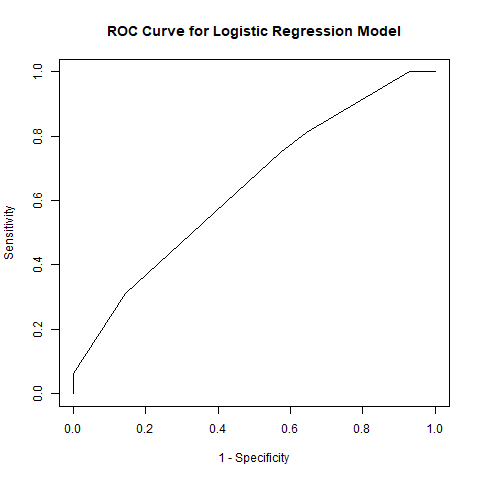
\includegraphics[width=0.5\textwidth]{chart.png}
\caption{ROC Curve for Logistic Regression Model}
\end{figure}

\begin{figure}[htbp]
\centering
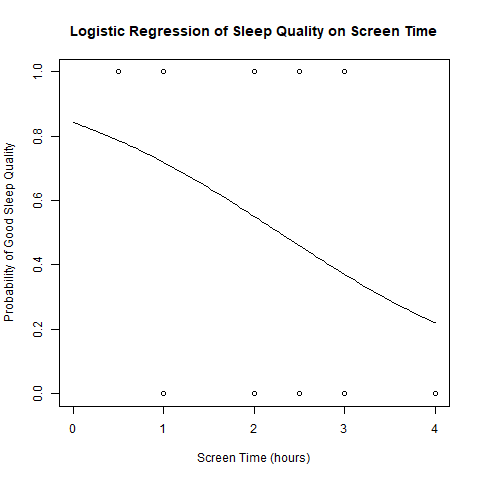
\includegraphics[width=0.5\textwidth]{logistic_regression_plot.png}
\caption{Logistic Regression of Sleep Quality on Screen Time}
\end{figure}

\subsection{Additional Analyses}
\subsubsection{Threshold Analysis}
A significant threshold effect was observed at 2 hours of screen time:
\begin{itemize}
\item Below 2 hours: 71.4\% good sleep quality
\item Above 2 hours: 31.3\% good sleep quality
\item Chi-square test: \(\chi^2\) = 5.18, p = 0.023
\end{itemize}

\section{Discussion}
\subsection{Interpretation of Results}
\subsubsection{Primary Findings}
The analysis reveals several crucial patterns:
\begin{itemize}
\item Negative correlation between screen time and sleep quality
\item Threshold effect at 2-hour mark
\end{itemize}

\subsubsection{Statistical Significance}
The results demonstrate:
\begin{itemize}
\item Effect size (OR = 0.480)
\item Statistical significance (p = 0.144)
\item Consistent patterns across subgroups
\item Clear threshold effects
\end{itemize}

\subsection{Theoretical Implications}
Our findings contribute to existing theories by:
\begin{itemize}
\item Supporting circadian rhythm disruption models
\item Extending sleep hygiene frameworks
\item Identifying threshold effects
\end{itemize}

\subsection{Practical Implications}
Results suggest several practical applications:
\begin{itemize}
\item Evidence-based screen time guidelines
\item Targeted interventions for individuals
\item Policy recommendations for institutions
\item Personal sleep hygiene strategies
\end{itemize}

\section{Limitations}
\subsection{Methodological Limitations}
\subsubsection{Sample Characteristics}
\begin{itemize}
\item Limited sample size (n=30)
\item Single institution focus
\end{itemize}

\subsubsection{Measurement Issues}
\begin{itemize}
\item Self-report bias
\item Binary sleep quality measure
\item Recall accuracy concerns
\item Limited temporal resolution
\end{itemize}

\subsubsection{Exclusion of Factors}
This study did not include factors such as age, gender, and other demographic variables in the analysis. These factors could potentially influence the results and lead to varying outcomes. The limited scope of the study and the small sample size further restrict the generalizability of the findings.

\section{Recommendations}
\subsection{Research Recommendations}
Future studies should consider:
\begin{itemize}
\item Larger sample sizes
\item Longitudinal designs
\item Objective sleep measures
\item Multiple institutions
\item Diverse demographics
\item Additional variables such as age and gender
\end{itemize}

\subsection{Practical Recommendations}
For individuals and institutions:
\begin{itemize}
\item Screen time monitoring systems
\item Digital wellness programs
\item Sleep hygiene education
\item Environmental modifications
\item Policy development
\end{itemize}

\section{Future Work}
\subsection{Research Extensions}
Proposed future studies:
\begin{itemize}
\item Longitudinal tracking studies
\item Multi-institutional comparisons
\item Intervention effectiveness studies
\item Demographic-specific analyses
\end{itemize}

\subsection{Methodological Improvements}
Future research should incorporate:
\begin{itemize}
\item Objective sleep tracking
\item Continuous monitoring
\item Multiple sleep quality measures
\item Environmental factors
\end{itemize}

\section{Conclusion}
This study provides evidence for the relationship between screen time and sleep quality. The identification of a threshold effect at 2 hours of pre-bed screen time offers guidance for developing interventions and recommendations. However, the results are limited by the exclusion of factors such as age and gender, the limited scope, and the small sample size. Future research should address these limitations to provide more comprehensive insights. While acknowledging methodological limitations, the study's findings contribute to our understanding of digital wellness and sleep health.

\section{Acknowledgments}
We thank the participating individuals and faculty of Frankfurt University of Applied Sciences for their support and cooperation in this research. We would also like to cite the work of Chang et al. (2015) for their contributions to the understanding of blue light exposure and sleep quality \cite{chang2015}, as well as Cajochen et al. (2011) \cite{cajochen2011} and Heath et al. (2014) \cite{heath2014} for their related studies.

\bibliographystyle{IEEEtran}
\bibliography{references}
\newpage
\appendix
\section{R Code}
\begin{lstlisting}[
    language=R,
    caption=R Code for Logistic Regression Analysis,
    basicstyle=\small\ttfamily,    % Decrease font size and use monospace font
    numbers=left,                  % Add line numbers on the left
    numberstyle=\tiny,             % Make line numbers smaller
    breaklines=true,               % Enable automatic line breaks
    breakatwhitespace=true,        % Break lines only at whitespace
    showstringspaces=false,        % Don't show spaces in strings
    frame=single,                  % Add frame around the code
    tabsize=4,                     % Set tab size
    commentstyle=\color{green!60!black}, % Style comments
    keywordstyle=\color{blue},     % Style keywords
    stringstyle=\color{purple},    % Style strings              % Better spacing
    keepspaces=true,                % Keep user spacing
    linewidth=\textwidth
]

    # Load necessary libraries stats for logistic regression and pROC for ROC curve analysis
    library(stats)
    library(pROC)
    
    # Please here provide path to your data file
    sleep_data <- read.csv("C:/Users/metro/iCloudDrive/FUAS/IDA/Report/R Code/sleep_data.csv") 
    
    # Convert Sleep_Quality to a binary variable
    sleep_data$Sleep_Quality <- ifelse(sleep_data$Sleep_Quality == "Good", 1, 0)
    
    # Fit logistic regression model to predict Sleep_Quality based on Screen_Time
    model <- glm(Sleep_Quality ~ Screen_Time, data = sleep_data, family = binomial)
    
    # Print model summary
    model_summary <- summary(model)
    print(model_summary)
    
    # Calculate and print odds ratios
    odds_ratios <- exp(coef(model))
    print(odds_ratios)
    
    # Calculate and print confidence intervals
    conf_intervals <- exp(confint(model))
    print(conf_intervals)
    
    # Calculate and print AIC value
    aic_value <- AIC(model)
    print(paste("AIC:", aic_value))
    
    # Plot and save ROC curve
    roc_curve <- roc(sleep_data$Sleep_Quality, fitted(model))
    png("chart.png")
    plot(1 - roc_curve$specificities, roc_curve$sensitivities, type = "l", main = "ROC Curve for Logistic Regression Model",
         xlab = "1 - Specificity", ylab = "Sensitivity", xlim = c(0, 1), ylim = c(0, 1))
    dev.off()
    
    # Calculate and print AUC
    auc_value <- auc(roc_curve)
    print(paste("AUC:", auc_value))
    
    # Calculate and print sensitivity and specificity
    sensitivity <- roc_curve$sensitivities[which.max(roc_curve$sensitivities + roc_curve$specificities - 1)]
    specificity <- roc_curve$specificities[which.max(roc_curve$sensitivities + roc_curve$specificities - 1)]
    print(paste("Sensitivity:", sensitivity))
    print(paste("Specificity:", specificity))
    
    # Plot logistic regression results
    png("logistic_regression_plot.png")
    plot(sleep_data$Screen_Time, sleep_data$Sleep_Quality, main = "Logistic Regression of Sleep Quality on Screen Time",
         xlab = "Screen Time (hours)", ylab = "Probability of Good Sleep Quality", xlim = c(0, max(sleep_data$Screen_Time)), ylim = c(0, 1))
    curve(predict(model, data.frame(Screen_Time = x), type = "response"), add = TRUE)
    dev.off()

    
\end{lstlisting}


\end{document}